%=============================
%  TERCER CAPITULO
%=============================
\chapter{Resultados}
\label{cap3}

En este capitulo escribir el resultado de su investigación científica...

A continuación se muestra algunas secciones en los que puede dividir sus resultados obtenidos.

\section{Análisis Estacional de las precipitaciones}

Lorem ipsum dolor sit amet, consectetur adipiscing elit. Aliquam ultricies lacinia euismod. Nam tempus risus in dolor rhoncus in interdum enim tincidunt. Donec vel nunc neque. In condimentum ullamcorper quam non consequat. Fusce sagittis tempor feugiat. Fusce magna erat, molestie eu convallis ut, tempus sed arcu. Quisque molestie, ante a tincidunt ullamcorper, sapien enim dignissim lacus, in semper nibh erat lobortis purus. Integer dapibus ligula ac risus convallis pellentesque. Lorem ipsum dolor sit amet, consectetur adipiscing elit. Aliquam ultricies lacinia euismod. Nam tempus risus in dolor rhoncus in interdum enim tincidunt. Donec vel nunc neque. In condimentum ullamcorper quam non consequat. Fusce sagittis tempor feugiat. Fusce magna erat, molestie eu convallis ut, tempus sed arcu. Quisque molestie, ante a tincidunt ullamcorper, sapien enim dignissim lacus, in semper nibh erat lobortis purus. Integer dapibus ligula ac risus convallis pellentesque.

\section{Análisis estacional de la temperatura de superficie del mar}

Lorem ipsum dolor sit amet, consectetur adipiscing elit. Aliquam ultricies lacinia euismod. Nam tempus risus in dolor rhoncus in interdum enim tincidunt. Donec vel nunc neque. In condimentum ullamcorper quam non consequat. Fusce sagittis tempor feugiat. Fusce magna erat, molestie eu convallis ut, tempus sed arcu. Quisque molestie, ante a tincidunt ullamcorper, sapien enim dignissim lacus, in semper nibh erat lobortis purus. Integer dapibus ligula ac risus convallis pellentesque.

Lorem ipsum dolor sit amet, consectetur adipiscing elit. Aliquam ultricies lacinia euismod. Nam tempus risus in dolor rhoncus in interdum enim tincidunt. Donec vel nunc neque. In condimentum ullamcorper quam non consequat. Fusce sagittis tempor feugiat. Fusce magna erat, molestie eu convallis ut, tempus sed arcu. Integer dapibus ligula ac risus convallis pellentesque. La Figura \ref{fig-enso} muestra la influencia del ENSO en las tasas de precipitación que ocurren sobre América del Sur. 

\begin{figure}[H]
\centering
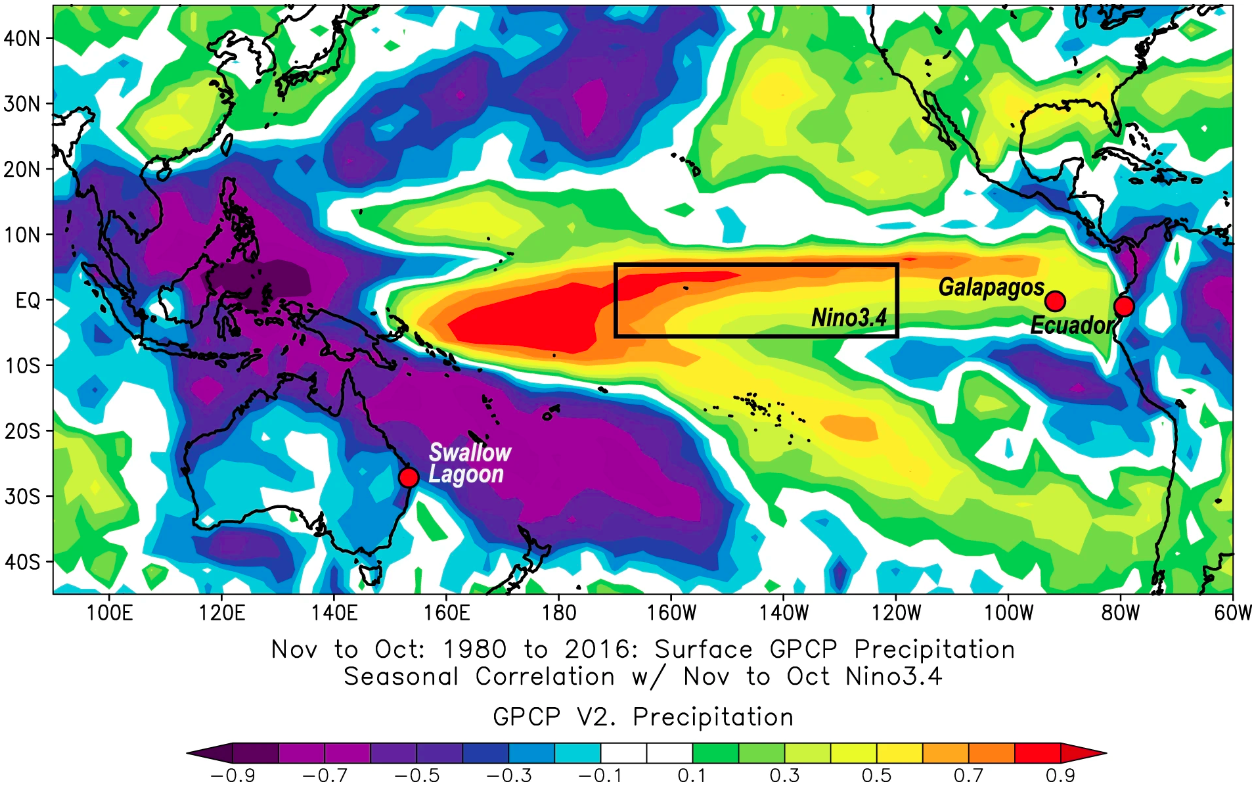
\includegraphics[width=1.0\textwidth]{Figuras/enso.png}
\vspace{-0.5cm}
\caption{Influencia del ENSO en la precipitación de América del Sur.}
\textbf{Fuente:} Adaptado de \cite{barr2019}.
\label{fig-enso}
\end{figure}

Segunda alternativa de colocar la leyenda y la fuente se muestra en la Figura~\ref{fig-enso2}:


\begin{figure}[H]
\centering
\caption{Influencia del ENSO en la precipitación de América del Sur.}
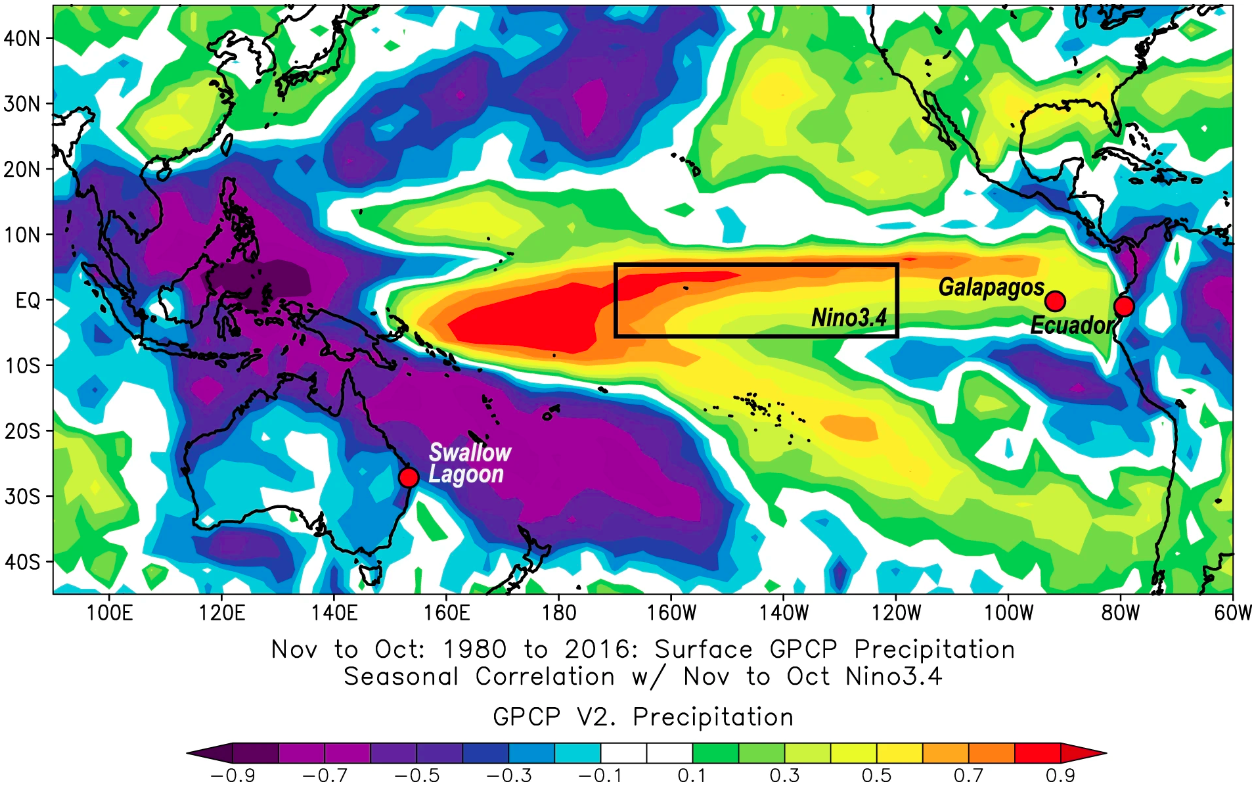
\includegraphics[width=1.0\textwidth]{Figuras/enso.png}
\vspace{-0.5cm}
\textbf{Fuente:} Adaptado de \cite{barr2019}.
\label{fig-enso2}
\end{figure}

Tercera alternativa de colocar la leyenda y la fuente se muestra en la Figura~\ref{fig-enso3}:

\begin{figure}[H]
\centering
\caption{Influencia del ENSO en la precipitación de América del Sur.}
\copyrightbox[b]{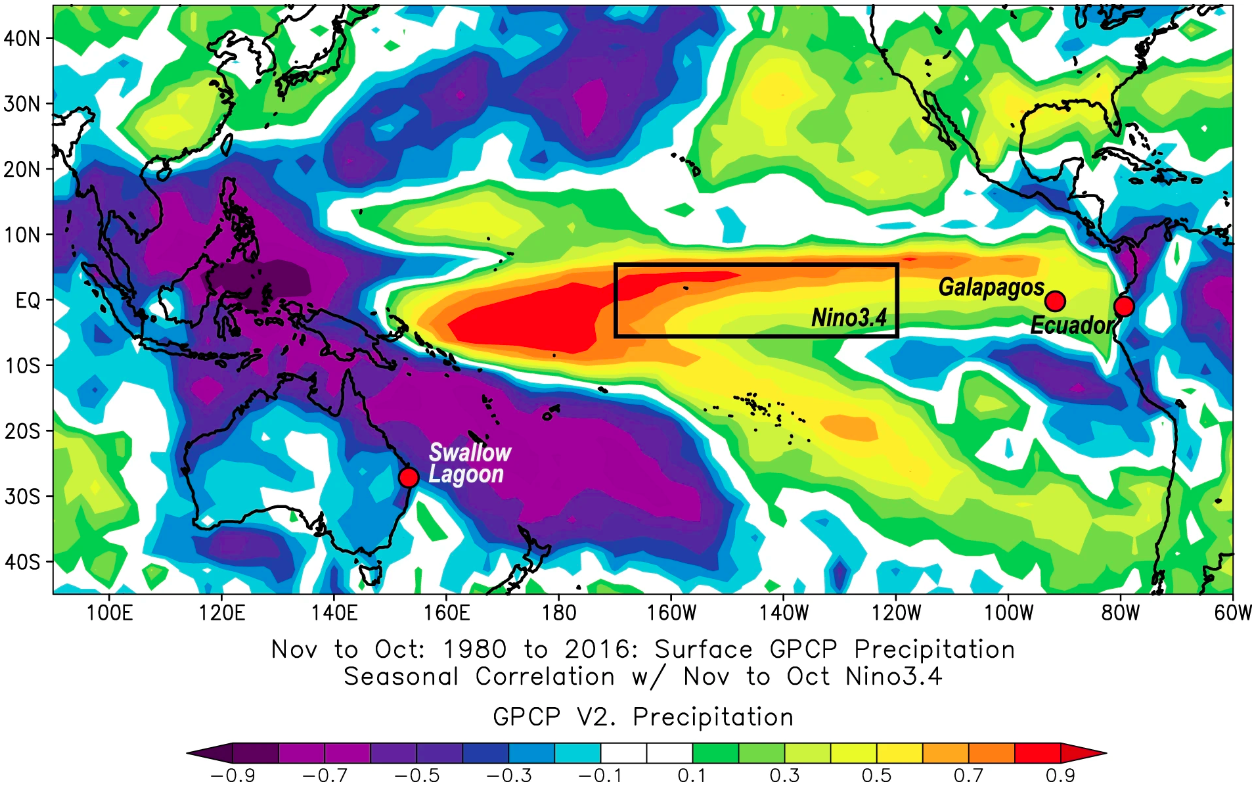
\includegraphics[width=1.0\linewidth]{Figuras/enso.png}}%
                {Fuente: Adaptado de \cite{barr2019}.}
\label{fig-enso3}
\end{figure}